\everymath{\displaystyle}
\documentclass{beamer}
% \documentclass[handout]{beamer}

%\usepackage[pdftex]{color,graphicx}
\usepackage{amsmath,amssymb,amsfonts}

\mode<presentation>
{
  % \usetheme{Darmstadt}
  % \usetheme[hideothersubsections]{Hannover}
  % \usetheme[hideothersubsections]{Goettingen}
  \usetheme[hideothersubsections, right]{Berkeley}

  \usecolortheme{seahorse}
  % \usecolortheme{dolphin}
  \usecolortheme{rose}
  % \usecolortheme{orchid}

  \useinnertheme[shadow]{rounded}

  \setbeamercovered{transparent}
  % or whatever (possibly just delete it)
}

\mode<handout>{
  \setbeamercolor{background canvas}{bg=black!5}
  \usepackage{pgfpages}
  \pgfpagesuselayout{4 on 1}[a4paper,border shrink=5mm, landscape]
}

\usepackage[brazilian]{babel}
% or whatever

% \usepackage[latin1]{inputenc}
\usepackage[utf8]{inputenc}
% or whatever

\usepackage{times}
%\usepackage[T1]{fontenc}
% Or whatever. Note that the encoding and the font should match. If T1
% does not look nice, try deleting the line with the fontenc.


\title%[] % (optional, use only with long paper titles)
{Variabilidade}

\subtitle
{Incertezas de dados numéricos} % (optional)

\author%[] % (optional, use only with lots of authors)
{Felipe Figueiredo}% \and S.~Another\inst{2}}
% - Use the \inst{?} command only if the authors have different
%   affiliation.

\institute[] % (optional, but mostly needed)
{
}
  % \inst{1}%
  % Department of Computer Science\\
  % University of Somewhere
  % \and
  % \inst{2}%
  % Department of Theoretical Philosophy\\
  % University of Elsewhere}
% - Use the \inst command only if there are several affiliations.
% - Keep it simple, no one is interested in your street address.

\date%[] % (optional)
{}

% \subject{Talks}
% This is only inserted into the PDF information catalog. Can be left
% out. 



% If you have a file called "university-logo-filename.xxx", where xxx
% is a graphic format that can be processed by latex or pdflatex,
% resp., then you can add a logo as follows:

\pgfdeclareimage[height=1.6cm]{university-logo}{../logo}
\logo{\pgfuseimage{university-logo}}



% Delete this, if you do not want the table of contents to pop up at
% the beginning of each subsection:
\AtBeginSubsection[]
%\AtBeginSection[]
{
  \begin{frame}<beamer>{Sumário}
    \tableofcontents[currentsection,currentsubsection]
  \end{frame}
}


% If you wish to uncover everything in a step-wise fashion, uncomment
% the following command: 

% \beamerdefaultoverlayspecification{<+->}


\begin{document}

\begin{frame}
  \titlepage
\end{frame}

\begin{frame}{Sumário}
  \tableofcontents
  % You might wish to add the option [pausesections]
\end{frame}


%% Template
% \section{}

% \subsection{}

% \begin{frame}{}
%   \begin{itemize}
%   \item 
%   \end{itemize}
% \end{frame}

% \begin{frame}
%   \begin{columns}
%     \begin{column}{5cm}
%     \end{column}
%     \begin{column}{5cm}
%     \end{column}
%   \end{columns}
% \end{frame}

% \begin{frame}{}
%   \includegraphics[height=0.4\textheight]{file1}
%   \includegraphics[height=0.4\textheight]{file2}
%   \includegraphics[height=0.4\textheight]{file3}
%   \begin{figure}
%     \caption{}
%   \end{figure}
% \end{frame}

% \begin{frame}{}
%   \begin{definition}
%   \end{definition}
%   \begin{example}
%   \end{example}
%   \begin{block}{Exercício}
%   \end{block}
% \end{frame}

\section{O desvio padrão}

\begin{frame}{Medidas Sumárias}
  \begin{itemize}
  \item Medidas sumárias resumem a informação contida nos dados em um
    pequeno conjunto de números.
  \item Medidas sumárias de \alert{populações} se chamam
    \alert{parâmetros}, e são representadas por letras gregas ($\mu$, $\sigma^2$, $\sigma$, etc).
  \item Medidas sumárias de \alert{amostras} se chamam \alert{estatísticas} e são representadas por letras comuns ($\bar{x}$, $s^2$, $s$, etc).
  \item {\em Geralmente trabalhamos com estatísticas descritivas.}
  \end{itemize}
\end{frame}

\begin{frame}{Medidas Sumárias}
  \begin{block}{Tipos de medidas sumárias}
    Os dois principais tipos de medidas sumárias utilizadas na literatura são:
    \begin{itemize}
    \item Medidas de Tendência Central
    \item Medidas de Variabilidade (ou Dispersão)
    \end{itemize}
  \end{block}
\end{frame}

\subsection{Fontes de Variabilidade}

\begin{frame}{Variabilidade em Medições}
  \begin{figure}
    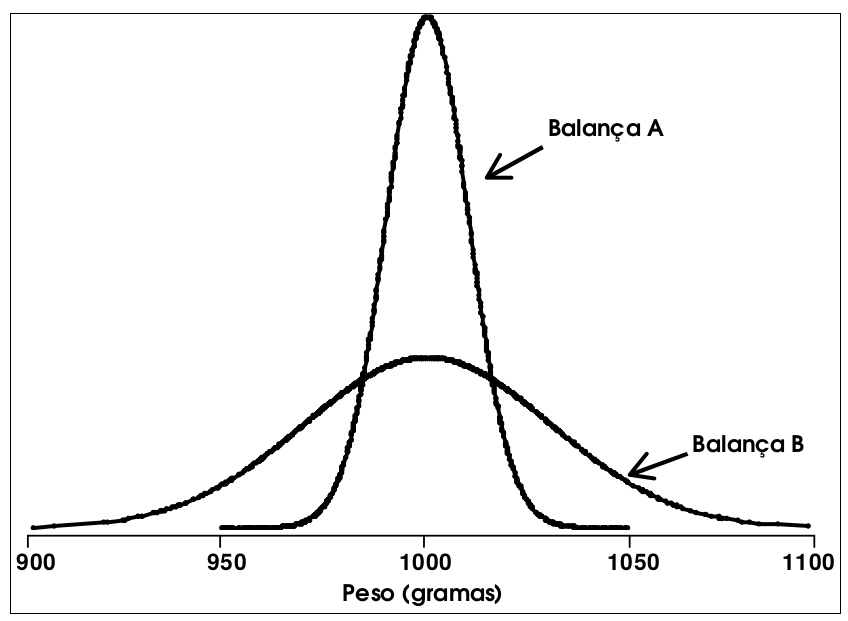
\includegraphics[height=0.7\textheight]{Desc_II/variancia}
    \caption{Variabilidade da medição de uma esfera metálica de
      1000g. Balança A, ``imprecisão'' de 50g, balança B,
      ``imprecisão'' de 100g (Fonte: Reis, Reis, 2002)}
  \end{figure}
\end{frame}

\begin{frame}{Fontes comuns de variabilidade}
  \begin{itemize}
  \item Imprecisão ou erro experimental
  \item Variabilidade biológica
  \item ``{\em Mancadas}'' experimentais
  \end{itemize}
  \begin{block}{Conceito de Erro na Estatística}
    No contexto acadêmico, {\bf erro} não tem o mesmo significado do cotidiano.

    \bigskip
    Erro se refere a todas as fontes de variabilidade acima.

    \bigskip
    Outro nome comum é {\bf dispersão} ({\em scatter}).
  \end{block}
\end{frame}

\subsection{Visualizando a variabilidade com histogramas}

\begin{frame}
  \begin{exampleblock}{Exemplo}
    100 estudantes de [{\em insira aqui um curso da área da saúde}] trabalharam em pares, e mediram a pressão sistólica de seu parceiro(a).

    Ao final do exercício, a turma obteve 100 valores de pressão sistólica.
  \end{exampleblock}
  \begin{block}{Pergunta}
    Como ``entender'' essa listagem de 100 números?
  \end{block}
\end{frame}

\begin{frame}{O histograma}
  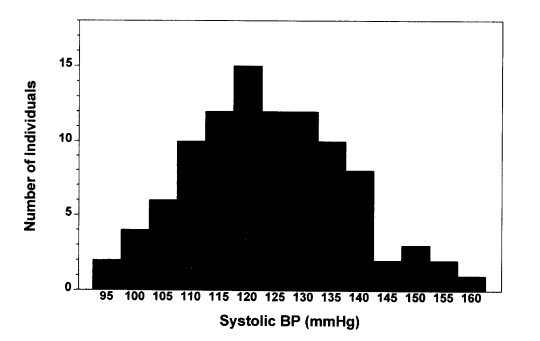
\includegraphics[height=\textheight]{Cap3/histograma1}
\end{frame}

\begin{frame}{Quantas barras?}
  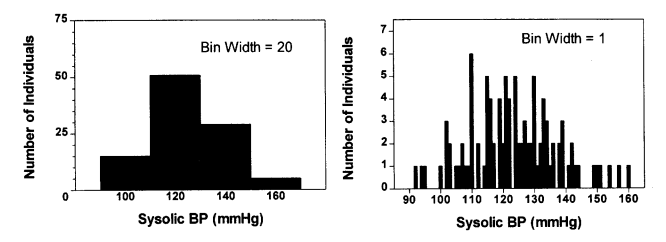
\includegraphics[width=\textwidth]{Cap3/histograma2}
\end{frame}

\subsection{Média e a mediana}

\begin{frame}{Média}
  \begin{example}
    Foram observados os seguintes níveis de colesterol de uma amostra
    de pacientes. Qual é o nível médio de colesterol nestes pacientes?

    \begin{columns}<1>
      \begin{column}{5cm}<1>
        \begin{tabular}{ccc}
          $x_1$ &=&142\\
          $x_2$ &=&144\\
          $x_3$ &=&176\\
          $x_4$ &=&203\\
          $x_5$ &=&134\\
          $x_6$ &=&191\\
        \end{tabular}
      \end{column}
      \begin{column}{5cm}<1>
        $\bar{x} = \frac{\sum x_i}{n} = \frac{990}{6} = 165$
      \end{column}
    \end{columns}
  \end{example}
\end{frame}


\begin{frame}{Mediana}
\begin{definition}
A mediana é o dado que ocupa a \alert{posição central} nos dados
    ordenados.
  \end{definition}
  \begin{itemize}
  \item Notação: $M_d$
  \item Divide o dataset ao meio
  % \item Mais robusta que a média na presença de {\it outliers}
  \item Costuma pertencer ao dataset
  \end{itemize}
\end{frame}

\begin{frame}{Mediana}
  \begin{itemize}
  \item Para se calcular a mediana, deve-se ordenar os dados.
  \item Encontrar o valor do meio se $n$ for ímpar.
  \item Encontrar a média dos dois valores do meio se $n$ for par.
  \end{itemize}
  \begin{example}
Conforme no exemplo anterior
    \begin{columns}
      \begin{column}{5cm}
        \begin{tabular}{ccc}
          $x_5$ &=&134\\
          $x_1$ &=&142\\
          $x_2$ &=&\alert{144}\\
          $x_3$ &=&\alert{176}\\
          $x_6$ &=&191\\
          $x_4$ &=&203\\
        \end{tabular}
      \end{column}
      \begin{column}{5cm}
        $M_d = \frac{144+176}{2}=160$
      \end{column}
    \end{columns}
  \end{example}
\end{frame}

\subsection{Quantificando com percentis}

\begin{frame}{O boxplot}
  \begin{columns}
    \begin{column}{7cm}
      \begin{itemize}
      \item {\em ``Caixa e bigodes''}
      \item A caixa representa os percentis de 25\% e 75\%
      \item Barra interna que representa a mediana (percentil 50\%)
      \item Barras verticais {\em indicam} a amplitude dos dados
        \begin{itemize}
        \item Mínimo e Máximo
        \item Regras para ``a maioria''
        \end{itemize}

      \end{itemize}
      \end{column}
      \begin{column}{5cm}
          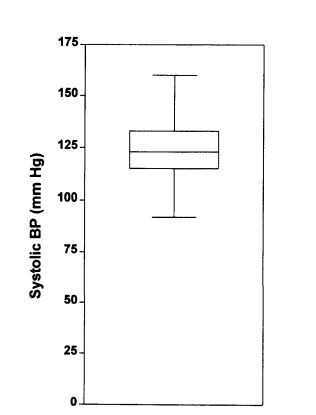
\includegraphics[height=\textheight]{Cap3/boxplot}
      \end{column}
  \end{columns}
\end{frame}

\begin{frame}{``Regras para a maioria''}
  \begin{figure}
    \centering
    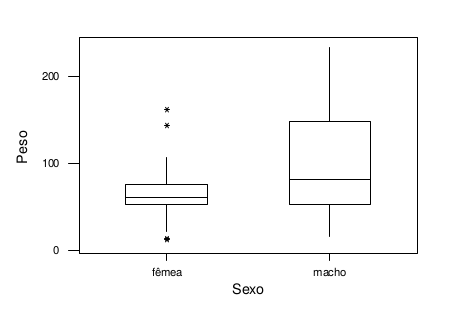
\includegraphics[height=0.7\textheight]{Desc_II/boxplot3}
    \caption{Boxplots para dois grupos de dados (Fonte: Reis, Reis,
      2002)}
  \end{figure}
\end{frame}

\subsection{Quantificando com variância e DP}

\subsection{N ou N-1?}

\subsection{Interpretação do DP}

\subsection{Exercícios}

\begin{frame}{Leitura pós-aula e exercícios selecionados}
  \begin{block}{Leitura obrigatória}
    Capítulo 3.

    Pular as seções:
    \begin{itemize}
    \item Calculando o DP numa calculadora
    \item Coeficiente de Variação (CV)
    \end{itemize}

  \end{block}
  \begin{itemize}
  \item Exercício 1
  \item Exercício 2
  \item Exercício 3 (R: 34.64503)
  \item Exercício 4 (R: 219.4131)
  \item Exercício 5
  \end{itemize}
\end{frame}

\end{document}
